\documentclass[12pt,a4paper]{article}

% Paquetes básicos
\usepackage[utf8]{inputenc}
\usepackage[T1]{fontenc}
\usepackage[english]{babel}
\usepackage{amsmath, amssymb}
%\usepackage{siunitx} 
\usepackage{graphicx}
\usepackage{float}
\usepackage{geometry}
\usepackage{xcolor}
\geometry{margin=2.5cm}
\usepackage{hyperref}
\usepackage{caption}
\usepackage{subcaption}
\usepackage{setspace}
\usepackage{multirow}
%\usepackage{minted}  
\usepackage{gensymb} 
\usepackage[backend=biber, style=ieee]{biblatex}
\usepackage[american, straightvoltages]{circuitikz}
\usepackage{csquotes}
\usepackage{indentfirst}
\addbibresource{references.bib}

\graphicspath{{Figures/}}
\onehalfspacing
\hypersetup{
    colorlinks  = true,
    linkcolor   = blue,    
    citecolor   = blue,
    urlcolor    = blue,
    filecolor   = blue
}

\begin{document}       
\renewcommand{\figureautorefname}{Fig.}
\renewcommand{\tableautorefname}{Tab.}
\renewcommand{\equationautorefname}{Eq.}


% Carátula personalizada
\begin{titlepage}
    \centering
    
\includegraphics[width=0.7\textwidth]{Fulgor Logo.png}\\[1.5cm]

    {\Large \textbf{FUNDACIÓN FULGOR} \\[0.5cm]}
    {\Large Undergrad CMOS Course} \\[0.5cm]

    \rule{\textwidth}{0.5pt} \\[0.5cm]
    {\Large \textbf{Homework N°5} \\[0.3cm]}
    \rule{\textwidth}{0.5pt} \\[1cm]
    
\begin{tabular}{l l}
    \textbf{Professors:} & Camilo Estevez.\\
                         & Ramón Sarmiento.\\
    \\
    \textbf{Student:}    & Monja, Ernesto Joaquín (43.873.728)\\
\end{tabular} \\[5cm]

{\centering Year 2026 \par}

\end{titlepage}



% Índice
\tableofcontents
\newpage



\section{Introduction}                                              \label{sec_1}
In this report, we will present the solutions to the analog \textit{CMOS} design exercises proposed in \textit{Homework 5} for the Undergrad \textit{CMOS} Course. Unless specific parameter values are provided within the problem statements, we will adhere to the general assumptions given in the assignment: 
\begin{equation}
    \begin{cases}
        \mu_{n} \cdot C_{ox} = 200 \, \left[\frac{\mu A}{V^{2}}\right] \\
        \mu_{p} \cdot C_{ox} = 100 \, \left[\frac{\mu A}{V^{2}}\right] \\
        V_{Th,n} = 0.4 \, [V] \\
        V_{Th,p} = -0.4 \, [V] \\
        \lambda = 0 \\
    \end{cases}
    \label{eq_1}
\end{equation}



\section{Exercise 1: Common-Source Bias Design}                     \label{sec_2}
\subsection{Problem Statement}                                      \label{sec_2.1}
The objective of this exercise is to design the common-source circuit shown in \autoref{fig:fig_1} for a drain current of $I_{D} = 1 \, [mA]$. 
\begin{figure}[H]
    \centering
    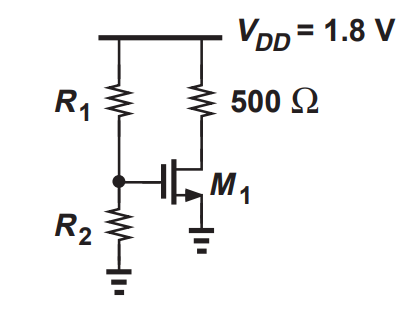
\includegraphics[width=0.35\linewidth]{Figures/Figure 1.PNG}
    \caption{Exercise 1 (Problem 7.2). \cite[p. 340]{b1}}
    \label{fig:fig_1}
\end{figure}

Given the transistor aspect ratio $W/L = 20/0.18$, we must calculate the bias resistors $R_{1}$ and $R_{2}$ such that the input impedance is at least $20 \,  [k\Omega]$. The technology parameters are $V_{DD} = 1.8 \, [V]$ and the rest must be followed according to \autoref{eq_1}


\subsection{Analysis and Resolution}                                \label{sec_2.2}
First, we assume the transistor $M_{1}$ operates in the saturation region. Since channel-length modulation is neglected ($\lambda = 0$), the drain current is given by:
\begin{equation}
    I_{D} = \frac{1}{2} \mu_{n} C_{ox} \frac{W}{L} (V_{GS} - V_{Th,n})^{2}
    \label{eq_2}
\end{equation}

Substituting the given values into the equation:
\begin{equation}
    1 \times 10^{-3} = \frac{1}{2} (200 \times 10^{-6}) \left(\frac{20}{0.18}\right) (V_{GS} - 0.4)^2
    \label{eq_3}
\end{equation}
\begin{equation}
    1 \times 10^{-3} \approx 11.11 \times 10^{-3} (V_{GS} - 0.4)^2 \implies (V_{GS} - 0.4)^2 \approx 0.09
    \label{eq_4}
\end{equation}

Solving for $V_{GS}$, we obtain $V_{GS} = 0.7 \, [V]$. Since the source is grounded, the gate voltage must be $V_G = 0.7 \, [V]$. Notice that the gate voltage is established by the $R_{1}$-$R_{2}$ voltage divider, this is:
\begin{equation}
    V_{G} = V_{DD} \frac{R_{2}}{R_{1} + R_{2}} \implies 0.7 = 1.8 \frac{R_{2}}{R_{1} + R_{2}}
    \label{eq_5}
\end{equation}

This yields the relationship shown in \autoref{eq_6}.
\begin{equation}
    R_{1} \approx 1.57 R_{2}
    \label{eq_6}
\end{equation}

To satisfy the input impedance requirement ($R_{in} \ge 20 \, [k\Omega]$), we evaluate the parallel combination of the bias resistors:
\begin{equation}
    R_{in} = R_{1}//R_{2} = \frac{1.57 R_{2} \cdot R_{2}}{1.57 R_{2} + R_{2}} \approx 0.611 R_{2}
    \label{eq_7}
\end{equation}
\begin{equation}
    0.611 R_{2} \ge 20 \, [k\Omega] \implies R_{2} \ge 32.73 \, [k\Omega]
    \label{eq_8}
\end{equation}

Selecting the minimum allowable values to satisfy the design constraint, we obtain:
\begin{equation}
    \begin{cases}
        R_{2} = 32.73 \, [k\Omega] \\
        R_{1} = 51.43\, [k\Omega]
    \end{cases}
    \label{eq_9}
\end{equation}

\textit{Note: To verify saturation, we check the drain voltage: $V_{D} = V_{DD} - I_{D} R_{D} = 1.8 - (1 \, [mA])(500 \, [\Omega])$ $= 1.3 \, [V]$. Since $V_{D} > V_{G} - V_{TH,n}$ ($1.3 \, [V] > 0.3 \, [V]$), the assumption holds true.}



\newpage
\section{Exercise 2: Common-Source with Source Degeneration}        \label{sec_3}
\subsection{Problem Statement}                                      \label{sec_3.1}
The circuit shown in \autoref{fig:fig_2} must be designed for a voltage drop of $V_{RS} = 200 \, [mV]$ across $R_{S}$.
\begin{figure}[H]
    \centering
    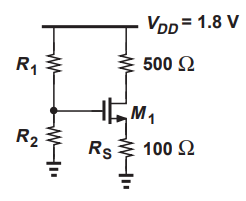
\includegraphics[width=0.3\linewidth]{Figures/Figure 2.PNG} 
    \caption{Exercise 2 (Problem 7.4). \cite[p. 341]{b1}}
    \label{fig:fig_2}
\end{figure}

The specific requirements are:
\begin{itemize}
    \item[(a)] Calculate the minimum allowable value of $W/L$ if $M_{1}$ must remain in saturation.
    \item[(b)] Calculate the required values of $R_{1}$ and $R_{2}$ if the input impedance must be at least $30 \, [k\Omega]$.
\end{itemize}

The technology parameters are given by \autoref{eq_1}, along with $V_{DD} = 1.8 \, [V]$, $R_{D} = 500 \, [\Omega]$, and $R_{S} = 100 \, [\Omega]$ as shown in \autoref{fig:fig_2}.


\subsection{Analysis and Resolution}                                \label{sec_3.2}
\subsubsection{Part (a): Minimum allowable value of W/L}            \label{sec_3.2.1}
First, we determine the drain current $I_{D}$ flowing through the circuit, which can be calculated using the specified voltage drop across the source resistor $R_{S}$:
\begin{equation}
    I_{D} = \frac{V_{RS}}{R_{S}} = \frac{0.2 \, [V]}{100 \, [\Omega]} = 2 \, [mA]
    \label{eq_10}
\end{equation}

To find the saturation condition, we need the drain voltage $V_{D}$ and the source voltage $V_{S}$. The source voltage is directly given as $V_{S} = V_{RS} = 0.2 \, [V]$. The drain voltage is calculated as follows:
\begin{equation}
    V_{D} = V_{DD} - I_{D} R_{D} = 1.8 - (2 \times 10^{-3})(500) = 0.8 \, [V]
    \label{eq_11}
\end{equation}

Consequently, the drain-to-source voltage $V_{DS}$ is:
\begin{equation}
    V_{DS} = V_{D} - V_{S} = 0.8 - 0.2 = 0.6 \, [V]
    \label{eq_12}
\end{equation}

For the transistor to remain in saturation, the condition $V_{DS} \ge V_{GS} - V_{Th,n}$ must be met. Thus, the maximum allowable overdrive voltage (The term $(V_{GS} - V_{Th,n})$ is defined as the overdrive voltage $V_{OV}$) for the transistor to stay in saturation is:
\begin{equation}
    V_{OV,max} = V_{DS} = 0.6 \, [V]
    \label{eq_13}
\end{equation}

Using the drain current equation for saturation (\autoref{eq_2}), we solve for the minimum aspect ratio $(W/L)_{min}$ using the maximum overdrive voltage:
\begin{equation}
    I_{D} = \frac{1}{2} \mu_{n} C_{ox} \left(\frac{W}{L}\right)_{min} V_{OV,max}^{2}
    \label{eq_14}
\end{equation}
\begin{equation}
    2 \times 10^{-3} = \frac{1}{2} (200 \times 10^{-6}) \left(\frac{W}{L}\right)_{min} (0.6)^{2}
    \label{eq_15}
\end{equation}
\begin{equation}
    2 \times 10^{-3} = 36 \times 10^{-6} \left(\frac{W}{L}\right)_{min} \implies \left(\frac{W}{L}\right)_{min} = \frac{2000}{36} \approx 55.56
    \label{eq_16}
\end{equation}


\subsubsection{Part (b): Required values of $R_{1}$ and $R_{2}$}    \label{sec_3.2.2}        
Using the maximum overdrive voltage established in \autoref{sec_3.2.1}, we calculate the required gate-to-source voltage $V_{GS}$:
\begin{equation}
    V_{GS} = V_{OV,max} + V_{Th,n} = 0.6 + 0.4 = 1.0 \, [V]
    \label{eq_17}
\end{equation}

Since $V_{S} = 0.2 \, [V]$, the absolute gate voltage $V_{G}$ referenced to ground must be:
\begin{equation}
    V_{G} = V_{GS} + V_{S} = 1.0 + 0.2 = 1.2 \, [V]
    \label{eq_18}
\end{equation}

The gate voltage is set by the resistive divider formed by $R_{1}$ and $R_{2}$:
\begin{equation}
    V_{G} = V_{DD} \frac{R_{2}}{R_{1} + R_{2}} \implies 1.2 = 1.8 \frac{R_{2}}{R_{1} + R_{2}}
    \label{eq_19}
\end{equation}
\begin{equation}
    1.2(R_{1} + R_{2}) = 1.8 R_{2} \implies 1.2 R_{1} = 0.6 R_{2} \implies R_{2} = 2 R_{1}
    \label{eq_20}
\end{equation}

The input impedance requirement is $R_{in} \ge 30 \, [k\Omega]$. Evaluating the parallel combination:
\begin{equation}
    R_{in} = R_{1}//R_{2} = \frac{R_{1} (2 R_{1})}{R_{1} + 2 R_{1}} = \frac{2}{3} R_{1}
    \label{eq_21}
\end{equation}
\begin{equation}
    \frac{2}{3} R_{1} \ge 30 \, [k\Omega] \implies R_{1} \ge 45 \, [k\Omega]
    \label{eq_22}
\end{equation}

Using the lower bound to satisfy the constraint, and applying the relationship from \autoref{eq_20}, we determine the required resistor values:
\begin{equation}
    \begin{cases}
        R_{1} = 45 \, [k\Omega] \\
        R_{2} = 90 \, [k\Omega]
    \end{cases}
    \label{eq_23}
\end{equation}



\newpage
\section{Exercise 3: Self-Biased Stage Design}                      \label{sec_4}
\subsection{Problem Statement}                                      \label{sec_4.1}
The self-biased stage shown in \autoref{fig:fig_3} must be designed for a drain current of $I_{D} = 1 \, [mA]$. 
\begin{figure}[H]
    \centering
    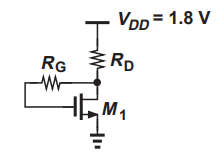
\includegraphics[width=0.25\linewidth]{Figures/Figure 3.PNG} 
    \caption{Exercise 3 (Problem 7.6). \cite[p. 341]{b1}}
    \label{fig:fig_3}
\end{figure}

If transistor $M_{1}$ must provide a transconductance of $g_{m} = 1/100 \, [\Omega^{-1}])$, we need to calculate the required value of $R_{D}$. The gate resistor $R_{G}$ must be neglected for \textit{DC} analysis. The general technology parameters from \autoref{eq_1} apply, along with $V_{DD} = 1.8 \, [V]$.


\subsection{Analysis and Resolution}                            \label{sec_4.2}
First, we determine the required transconductance $g_{m}$ in standard units:
\begin{equation}
    g_{m} = \frac{1}{100 \, [\Omega]} = 0.01 \, \left[\frac{A}{V}\right] = 10 \, \left[\frac{mA}{V}\right]
    \label{eq_24}
\end{equation}

In the saturation region, the transconductance can be expressed in terms of the drain current $I_{D}$ and the overdrive voltage $(V_{GS} - V_{Th,n})$:
\begin{equation}
    g_{m} = \frac{2 I_{D}}{V_{GS} - V_{Th,n}}
    \label{eq_25}
\end{equation}

By rearranging \autoref{eq_25}, we can solve for the required gate-to-source voltage $V_{GS}$:
\begin{equation}
    V_{GS} - V_{Th,n} = \frac{2 I_{D}}{g_{m}} = \frac{2 \times 10^{-3} \, [A]}{10 \times 10^{-3} \, [A/V]} = 0.2 \, [V]
    \label{eq_26}
\end{equation}
\begin{equation}
    V_{GS} = 0.2 \, [V] + V_{Th,n} = 0.2 \, [V] + 0.4 \, [V] = 0.6 \, [V]
    \label{eq_27}
\end{equation}

For the \textit{DC} bias analysis of this self-biased configuration, we must consider the voltage drop across the feedback resistor $R_{G}$. Since the \textit{DC} gate current of a \textit{MOSFET} is ideally zero ($I_{G} = 0$), there is no voltage drop across $R_{G}$. Therefore, the drain voltage $V_{D}$ is equal to the gate voltage $V_{G}$. Since the source is grounded ($V_{S} = 0$), we conclude that:
\begin{equation}
    V_{D} = V_{G} = V_{GS} = 0.6 \, [V]
    \label{eq_28}
\end{equation}

Finally, the required drain resistor $R_{D}$ can be calculated using \textit{Ohm's law}, given the voltage drop across it and the drain current flowing through it:
\begin{equation}
    R_{D} = \frac{V_{DD} - V_{D}}{I_{D}}
    \label{eq_29}
\end{equation}
\begin{equation}
    R_{D} = \frac{1.8 \, [V] - 0.6 \, [V]}{1 \times 10^{-3} \, [A]} = \frac{1.2 \, [V]}{1 \times 10^{-3} \, [A]} = 1.2 \, [k\Omega]
    \label{eq_30}
\end{equation}

Thus, the required value for the drain resistor is $R_{D} = 1.2 \, [k\Omega]$. Note that the condition $V_{DS} = V_{GS}$ inherently guarantees that the transistor operates in the saturation region, as $V_{DS} > V_{GS} - V_{Th,n}$ is strictly satisfied ($0.6 \, [V] > 0.2 \, [V]$).




\newpage
\section{Exercise 4: Common-Source Stage Analysis}                  \label{sec_5}
\subsection{Problem Statement}                                      \label{sec_5.1}
In the common-source stage shown in \autoref{fig:fig_4}, the transistor has an aspect ratio of $W/L = 30/0.18$ and channel-length modulation is neglected ($\lambda = 0$). 
\begin{figure}[H]
    \centering
    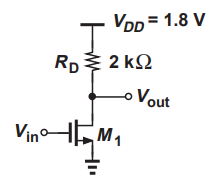
\includegraphics[width=0.25\linewidth]{Figures/Figure 4.PNG} 
    \caption{Exercise 4 (Problem 7.17). \cite[p. 342]{b1}}
    \label{fig:fig_4}
\end{figure}

We are tasked with determining:
\begin{itemize}
    \item[(a)] The gate voltage $V_{G}$ that yields a drain current of $I_{D} = 0.5 \, [mA]$, and verifying that $M_{1}$ operates in saturation.
    \item[(b)] The voltage gain $A_{v}$ of the stage under this bias condition.
\end{itemize}

The parameters given are $V_{DD} = 1.8 \, [V]$ and $R_{D} = 2 \, [k\Omega]$. We will use the general technology parameters from \autoref{eq_1}.


\subsection{Analysis and Resolution}                                \label{sec_5.2}
\subsubsection{Part (a): Gate Voltage and Saturation Verification}  \label{sec_5.2.1}
Assuming the transistor operates in the saturation region, the drain current is described by \autoref{eq_2}. We can rearrange this equation to solve for the required overdrive voltage $V_{OV} = (V_{GS} - V_{Th,n})$:
\begin{equation}
    V_{OV} = \sqrt{\frac{2 I_{D}}{\mu_{n} C_{ox} \left(\frac{W}{L}\right)}}
    \label{eq_31}
\end{equation}

Substituting the known values:
\begin{equation}
    V_{OV} = \sqrt{\frac{2 (0.5 \times 10^{-3})}{(200 \times 10^{-6}) \left(\frac{30}{0.18}\right)}} = \sqrt{\frac{10^{-3}}{(200 \times 10^{-6}) (166.67)}} = \sqrt{\frac{10^{-3}}{33.33 \times 10^{-3}}}
    \label{eq_32}
\end{equation}
\begin{equation}
    V_{OV} = \sqrt{0.03} \approx 0.173 \, [V]
    \label{eq_33}
\end{equation}

Since the source is grounded ($V_{S} = 0$), the gate-to-source voltage $V_{GS}$ is equal to the gate voltage $V_{G}$. Thus:
\begin{equation}
    V_{G} = V_{GS} = V_{OV} + V_{Th,n} = 0.173 \, [V] + 0.4 \, [V] = 0.573 \, [V]
    \label{eq_34}
\end{equation}

To verify that $M_{1}$ operates in saturation, we must ensure that $V_{DS} \ge V_{OV}$. The drain voltage $V_{D}$ is calculated by analyzing the voltage drop across $R_{D}$:
\begin{equation}
    V_{D} = V_{DD} - I_{D} R_{D} = 1.8 \, [V] - (0.5 \times 10^{-3} \, [A])(2 \times 10^{3} \, [\Omega]) = 1.8 \, [V] - 1.0 \, [V] = 0.8 \, [V]
    \label{eq_35}
\end{equation}

Since $V_{S} = 0$, $V_{DS} = 0.8 \, [V]$. Comparing $V_{DS}$ and $V_{OV}$:
\begin{equation}
    0.8 \, [V] > 0.173 \, [V] \implies V_{DS} > V_{OV}
    \label{eq_36}
\end{equation}

The condition is satisfied; therefore, $M_{1}$ operates in the saturation region.


\subsubsection{Part (b): Voltage Gain}                              \label{sec_5.2.2}
The small-signal voltage gain $A_{v}$ of a common-source stage with a resistive load and $\lambda = 0$ (implying output resistance $r_{o} \to \infty$) is given by:
\begin{equation}
    A_{v} = -g_{m} R_{D}
    \label{eq_37}
\end{equation}

First, we determine the transconductance $g_{m}$ of the transistor at the current bias point:
\begin{equation}
    g_{m} = \frac{2 I_{D}}{V_{OV}} = \frac{2 (0.5 \times 10^{-3} \, [A])}{0.173 \, [V]} = \frac{1 \times 10^{-3}}{0.173} \approx 5.77 \, \left[\frac{mA}{V}\right]
    \label{eq_38}
\end{equation}

Now, substituting $g_{m}$ and $R_{D}$ into the gain equation:
\begin{equation}
    A_{v} = -(5.77 \times 10^{-3} \, [A/V])(2000 \, [\Omega]) \approx -11.54 \, \left[\frac{V}{V}\right]
    \label{eq_39}
\end{equation}



\newpage
\section{Exercise 5: Common-Source Stage with Active Load}          \label{sec_6}
\subsection{Problem Statement}                                      \label{sec_6.1}
The common-source stage shown in \autoref{fig:fig_5} must provide a voltage gain of $|A_{v}| = 10$ with a bias current of $I_{D} = 0.5 \, [mA]$. 
\begin{figure}[H]
    \centering
    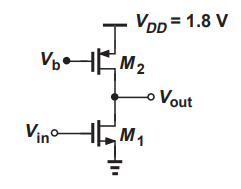
\includegraphics[width=0.25\linewidth]{Figures/Figure 5.PNG} 
    \caption{Exercise 5 (Problem 7.20). \cite[p. 343]{b1}}
    \label{fig:fig_5}
\end{figure}

For this problem, channel-length modulation must be considered, with parameters $\lambda_{1} = 0.1 \, [V^{-1}]$ and $\lambda_{2} = 0.15 \, [V^{-1}]$. We are asked to:
\begin{itemize}
    \item[(a)] Calculate the required aspect ratio $(W/L)_{1}$ of the input transistor $M_{1}$.
    \item[(b)] Determine the required bias voltage $V_{b}$ if $(W/L)_{2} = 20/0.18$.
\end{itemize}

General technology parameters apply defined in \autoref{eq_1} and \autoref{fig:fig_5}.


\subsection{Analysis and Resolution}                                \label{sec_6.2}
\subsubsection{Part (a): Required $(W/L)_{1}$}                      \label{sec_6.2.1}
The magnitude of the voltage gain for a common-source stage with an active \textit{PMOS} load is given by:
\begin{equation}
    |A_{v}| = g_{m1} (r_{o1} // r_{o2})
    \label{eq_40}
\end{equation}
where $g_{m1}$ is the transconductance of $M_{1}$, and $r_{o1}$ and $r_{o2}$ are the output resistances of $M_{1}$ and $M_{2}$, respectively.

First, we calculate the output resistances $r_{o1}$ and $r_{o2}$ using the bias current $I_{D}$:
\begin{equation}
    r_{o1} = \frac{1}{\lambda_{1} I_{D}} = \frac{1}{(0.1 \, [V^{-1}]) (0.5 \times 10^{-3} \, [A])} = 20 \, [k\Omega]
    \label{eq_41}
\end{equation}
\begin{equation}
    r_{o2} = \frac{1}{\lambda_{2} I_{D}} = \frac{1}{(0.15 \, [V^{-1}]) (0.5 \times 10^{-3} \, [A])} \approx 13.33 \, [k\Omega]
    \label{eq_42}
\end{equation}

The equivalent output resistance of the stage $R_{out}$ is the parallel combination of $r_{o1}$ and $r_{o2}$:
\begin{equation}
    R_{out} = r_{o1} // r_{o2} = \frac{20 \, [k\Omega] \times 13.33 \, [k\Omega]}{20 \, [k\Omega] + 13.33 \, [k\Omega]} = 8 \, [k\Omega]
    \label{eq_43}
\end{equation}

Given the required voltage gain $|A_{v}| = 10$, we can solve for the necessary transconductance $g_{m1}$:
\begin{equation}
    |A_{v}| = g_{m1} R_{out} \implies g_{m1} = \frac{10}{8000 \, [\Omega]} = 1.25 \, \left[\frac{mA}{V}\right]
    \label{eq_44}
\end{equation}

The transconductance of $M_{1}$ in saturation can also be expressed as:
\begin{equation}
    g_{m1} = \sqrt{2 \mu_{n} C_{ox} \left(\frac{W}{L}\right)_{1} I_{D}}
    \label{eq_45}
\end{equation}

Squaring both sides and solving for $(W/L)_{1}$:
\begin{equation}
    g_{m1}^{2} = 2 \mu_{n} C_{ox} \left(\frac{W}{L}\right)_{1} I_{D} \implies \left(\frac{W}{L}\right)_{1} = \frac{g_{m1}^{2}}{2 \mu_{n} C_{ox} I_{D}}
    \label{eq_46}
\end{equation}
\begin{equation}
    \left(\frac{W}{L}\right)_{1} = \frac{(1.25 \times 10^{-3})^{2}}{2 (200 \times 10^{-6}) (0.5 \times 10^{-3})} = \frac{1.5625 \times 10^{-6}}{200 \times 10^{-9}} \approx 7.81
    \label{eq_47}
\end{equation}


\subsubsection{Part (b): Required Bias Voltage $V_{b}$}             \label{sec_6.2.2}
To find the bias voltage $V_{b}$ at the gate of the \textit{PMOS} transistor $M_{2}$, we use its drain current equation. For \textit{DC} biasing purposes, we can neglect the small variations caused by channel-length modulation:
\begin{equation}
    I_{D} = \frac{1}{2} \mu_{p} C_{ox} \left(\frac{W}{L}\right)_{2} |V_{GS2} - V_{Th,p}|^{2}
    \label{eq_48}
\end{equation}

Substituting the known parameters:
\begin{equation}
    0.5 \times 10^{-3} = \frac{1}{2} (100 \times 10^{-6}) \left(\frac{20}{0.18}\right) |V_{GS2} - (-0.4)|^{2}
    \label{eq_49}
\end{equation}
\begin{equation}
    0.5 \times 10^{-3} = (50 \times 10^{-6}) (111.11) |V_{GS2} + 0.4|^{2} = 5.555 \times 10^{-3} |V_{GS2} + 0.4|^{2}
    \label{eq_50}
\end{equation}
\begin{equation}
    |V_{GS2} + 0.4|^{2} = \frac{0.5 \times 10^{-3}}{5.555 \times 10^{-3}} \approx 0.09 \, [V^{2}]
    \label{eq_51}
\end{equation}

Taking the square root, we obtain the absolute value of the overdrive voltage for the \textit{PMOS}:
\begin{equation}
    |V_{GS2} + 0.4| = \sqrt{0.09} = 0.3 \, [V]
    \label{eq_52}
\end{equation}

For a \textit{PMOS} device, the source-to-gate voltage $V_{SG2}$ must overcome the threshold voltage magnitude $|V_{Th,p}|$ to maintain operation:
\begin{equation}
    V_{SG2} = |V_{GS2} + 0.4| + |V_{Th,p}| = 0.3 \, [V] + 0.4 \, [V] = 0.7 \, [V]
    \label{eq_53}
\end{equation}

Since the source of $M_{2}$ is connected to $V_{DD}$, the bias voltage $V_{b}$ (which is the gate voltage $V_{G2}$) is calculated as:
\begin{equation}
    V_{SG2} = V_{DD} - V_{b} \implies 0.7 \, [V] = 1.8 \, [V] - V_{b}
    \label{eq_54}
\end{equation}
\begin{equation}
    V_{b} = 1.8 \, [V] - 0.7 \, [V] = 1.1 \, [V]
    \label{eq_55}
\end{equation}

Thus, the required bias voltage is $V_{b} = 1.1 \, [V]$.




\newpage
\section{Exercise 6: Common-Source Stage with Diode-Connected Load} \label{sec_7}
\subsection{Problem Statement}                                      \label{sec_7.1}
The objective of this final exercise is to design the circuit shown in \autoref{fig:fig_6} for a voltage gain of $|A_{v}| = 3$. 
\begin{figure}[H]
    \centering
    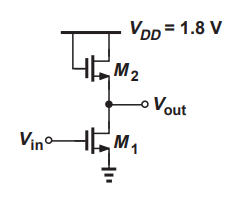
\includegraphics[width=0.25\linewidth]{Figures/Figure 6.PNG} 
    \caption{Exercise 6 (Problem 7.25). \cite[p. 344]{b1}}
    \label{fig:fig_6}
\end{figure}

Given the aspect ratio of the input transistor $(W/L)_{1} = 20/0.18$, we must determine the required aspect ratio of the diode-connected load $(W/L)_{2}$. We assume channel-length modulation is negligible ($\lambda = 0$). The standard technology parameters from \autoref{eq_1} apply.


\subsection{Analysis and Resolution}                                \label{sec_7.2}
For a common-source amplifier with a diode-connected \textit{PMOS} load, and neglecting channel-length modulation ($\lambda = 0 \implies r_{o} \to \infty$), the small-signal voltage gain $A_{v}$ is given by the ratio of the transconductances:
\begin{equation}
    A_{v} = -\frac{g_{m1}}{g_{m2}} \implies |A_{v}| = \frac{g_{m1}}{g_{m2}}
    \label{eq_56}
\end{equation}

The transconductance of a \textit{MOSFET} in saturation can be expressed in terms of the bias current $I_{D}$ and its physical parameters:
\begin{equation}
    g_{m} = \sqrt{2 \mu C_{ox} \left(\frac{W}{L}\right) I_{D}}
    \label{eq_57}
\end{equation}

Substituting the transconductance expressions for both $M_{1}$ (\textit{NMOS}) and $M_{2}$ (\textit{PMOS}) into the gain equation:
\begin{equation}
    |A_{v}| = \frac{\sqrt{2 \mu_{n} C_{ox} (W/L)_{1} I_{D}}}{\sqrt{2 \mu_{p} C_{ox} (W/L)_{2} I_{D}}}
    \label{eq_58}
\end{equation}

Since both transistors are connected in series, they share the exact same \textit{DC} drain current ($I_{D1} = I_{D2} = I_{D}$). We can cancel $\sqrt{2}$ and $\sqrt{I_{D}}$ from the numerator and denominator:
\begin{equation}
    |A_{v}| = \sqrt{\frac{\mu_{n} C_{ox} (W/L)_{1}}{\mu_{p} C_{ox} (W/L)_{2}}}
    \label{eq_59}
\end{equation}

Now, we square both sides to isolate and solve for the unknown aspect ratio $(W/L)_{2}$:
\begin{equation}
    |A_{v}|^{2} = \frac{\mu_{n} C_{ox} (W/L)_{1}}{\mu_{p} C_{ox} (W/L)_{2}}
    \label{eq_60}
\end{equation}
\begin{equation}
    \left(\frac{W}{L}\right)_{2} = \frac{\mu_{n} C_{ox} (W/L)_{1}}{\mu_{p} C_{ox} |A_{v}|^{2}}
    \label{eq_61}
\end{equation}

Substituting the known values ($|A_{v}| = 3$, $\mu_{n} C_{ox} = 200 \, [\mu A/V^{2}]$, $\mu_{p} C_{ox} = 100 \, [\mu A/V^{2}]$, and $(W/L)_{1} = 20/0.18$):
\begin{equation}
    \left(\frac{W}{L}\right)_{2} = \frac{200 \times 10^{-6} \left(\frac{20}{0.18}\right)}{100 \times 10^{-6} (3)^{2}}
    \label{eq_62}
\end{equation}
\begin{equation}
    \left(\frac{W}{L}\right)_{2} = \frac{2 \left(\frac{20}{0.18}\right)}{9} = \frac{40}{0.18 \times 9} = \frac{40}{1.62} \approx 24.69
    \label{eq_63}
\end{equation}

Therefore, the required aspect ratio for the \textit{PMOS} diode-connected load is approximately $24.69$.



\newpage
\section{Conclusion}                                                \label{sec_8}
In conclusion, this report successfully presented the step-by-step design and analysis of fundamental analog \textit{CMOS} amplifier stages, primarily focusing on various configurations of the common-source topology. Through the resolution of these six exercises, theoretical concepts were applied to determine appropriate \textit{DC} bias conditions, verify transistor operation in the saturation region, and calculate key small-signal performance metrics such as voltage gain and input impedance. 

The progression from simple resistive loads and source degeneration to more complex active and diode-connected \textit{PMOS} loads provided valuable insight into the practical trade-offs of analog \textit{IC} design. Furthermore, the systematic application of the provided technology parameters ensured a rigorous and consistent mathematical evaluation across all the proposed circuits, reinforcing the analytical foundation required for advanced \textit{CMOS} design.



\printbibliography[heading=bibintoc, title={9 \, Bibliography}]
\end{document}
